\documentclass{article}
% translate with >> pdflatex -shell-escape <file>

% This file is an extract of the PGFPLOTS manual, copyright by Christian Feuersaenger.
% 
% Feel free to use it as long as you cite the pgfplots manual properly.
%
% See
%   http://pgfplots.sourceforge.net/pgfplots.pdf
% for the complete manual.
%
% Any required input files (for <plot table> or <plot file> or the table package) can be downloaded
% at
% http://www.ctan.org/tex-archive/graphics/pgf/contrib/pgfplots/doc/latex/
% and
% http://www.ctan.org/tex-archive/graphics/pgf/contrib/pgfplots/doc/latex/plotdata/

\usepackage{pgfplots}
\pgfplotsset{compat=newest}

\pagestyle{empty}

\begin{document}
% the same as above for 3D ...
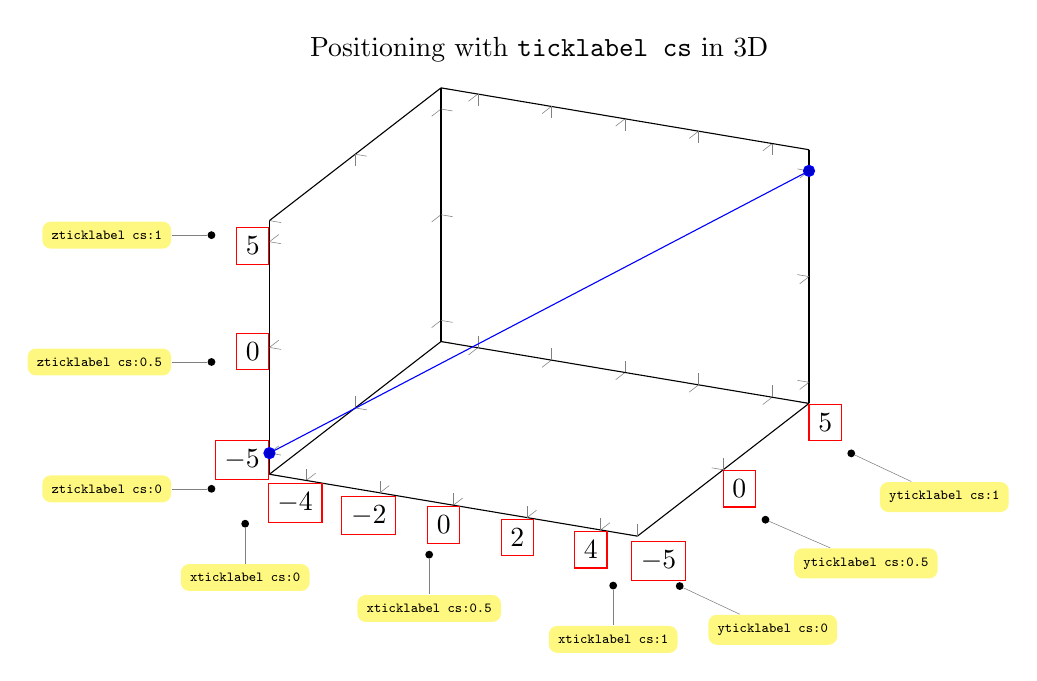
\begin{tikzpicture}
	\tikzset{
		every pin/.style={fill=yellow!50!white,rectangle,rounded corners=3pt,font=\tiny},
		small dot/.style={fill=black,circle,scale=0.3}
	}
	\begin{axis}[
		ticklabel style={draw=red},
		clip=false,
		title=Positioning with \texttt{ticklabel cs} in 3D
	]
	\addplot3 coordinates {(-5,-5,-5) (5,5,5)};

	\node[small dot,pin=-90:{\texttt{xticklabel cs:0}}]     at (xticklabel cs:0) {};
	\node[small dot,pin=-90:{\texttt{xticklabel cs:0.5}}]   at (xticklabel cs:0.5) {};
	\node[small dot,pin=-90:{\texttt{xticklabel cs:1}}]     at (xticklabel cs:1) {};

	\node[small dot,pin=-45:{\texttt{yticklabel cs:0}}]     at (yticklabel cs:0) {};
	\node[small dot,pin=-45:{\texttt{yticklabel cs:0.5}}]   at (yticklabel cs:0.5) {};
	\node[small dot,pin=-45:{\texttt{yticklabel cs:1}}]     at (yticklabel cs:1) {};

	\node[small dot,pin=180:{\texttt{zticklabel cs:0}}]     at (zticklabel cs:0) {};
	\node[small dot,pin=180:{\texttt{zticklabel cs:0.5}}]   at (zticklabel cs:0.5) {};
	\node[small dot,pin=180:{\texttt{zticklabel cs:1}}]     at (zticklabel cs:1) {};
	\end{axis}
\end{tikzpicture}
\end{document}
